\documentclass[a4paper,12pt,fleqn]{article}
\usepackage[T1]{fontenc}
\usepackage{ucs}
\usepackage[utf8x]{inputenc}
\usepackage{ngerman}
\usepackage[ngerman]{babel}
\usepackage{lastpage}
\usepackage[pdftex]{color,graphicx}
\usepackage{listings}
\usepackage{pdflscape}
\usepackage{longtable}
\usepackage[inner=2cm,outer=2cm,top=1cm,bottom=1.5cm,includeheadfoot]{geometry}
\usepackage{fancyhdr}
\usepackage{url}
\usepackage{draftwatermark}
\usepackage{booktabs}
\usepackage{blindtext} 
\usepackage{framed} 
\usepackage{xcolor} 
\colorlet{shadecolor}{black} 

\usepackage{enumitem}

\SetWatermarkText{Vertraulich}
\SetWatermarkScale{4}
\SetWatermarkLightness{0.9}

\usepackage{pgfgantt}
\usepackage{amsmath,amssymb,amsfonts,amstext}
\usepackage{floatflt}
\usepackage{tikz}
\usetikzlibrary[arrows,snakes,backgrounds,shapes]
\usetikzlibrary{through}
\usetikzlibrary{calc}
\usepackage{caption}
\usepackage{subcaption}

% highlighting
\usepackage{xcolor,soul}

%---- PageLayout
\pagestyle{fancy}

\setlength{\headsep}{10mm}

\usepackage{eso-pic}

%----------------------------------------------------------------------------
% HEADER --------------------------------------------------------------------
%----------------------------------------------------------------------------
\fancyhead[R]{
  
\includegraphics[width=100pt,keepaspectratio]{img/amedo2012.png}
}

\fancyhead[C]{ Wochenbericht KW 25 }

\fancyhead[L]{
  \begin{tabular}[b]{l}
  Christoph Gnip\\
  Projekt: PRPS-Evolution
  \end{tabular}
}

%Linie oben
\renewcommand{\headrulewidth}{0.5pt}
%----------------------------------------------------------------------------

%----------------------------------------------------------------------------
%----------------------------------------------------------------------------
%----------------------------------------------------------------------------
\fancyfoot[L]{Stand: \today}
\fancyfoot[C]{ EXTERN }
\fancyfoot[R]{\thepage{} von \pageref{LastPage}}

% Linie unten
\renewcommand{\footrulewidth}{0.5pt}
%----------------------------------------------------------------------------

% Import Macros  ------------------------------------------------------------
\newcommand\nn{\newline\newline}

%----------------------------------------------------------------------------
% Start the Document --------------------------------------------------------
%----------------------------------------------------------------------------
\begin{document}

\setlength{\headheight}{36pt}

\begin{titlepage}


%- the Title page --------------------------------------------------------
\begin{center}
%\vspace*{2.5cm}
{\Huge \textbf{Wochenbericht KW 25}\par}
\vspace{1cm}
{\Huge 18.6. - 23.6.2013\par}
\vspace{1cm}
{\Huge Projektwoche: 9\par}

\vspace{2cm}

\large{Erstellt durch}\\
\Large{\textbf{Christoph Gnip}}


\vspace{4cm}

\Large{\textbf{Extern}}

\vfill

{\normalsize Fachbereich Elektrotechnik und angewandte Naturwissenschaften\\
Westfälische Hochschule\\[2ex]Juni 2013}


\end{center}
\newpage

\end{titlepage}

%- Section 1 ----------------------------------------------------------------
\section[Allgemeines]{Allgemeines}
%
%- Section 2 ------s----------------------------------------------------------
\section[Fortschritt]{Projektfortschritt}
%
In der ersten Wochenhälfte wurden weitere Untersuchungen an dem Umgestellten Modell durchgeführt. Die Normierung der Eingangsparameter wurde entsprechend gewählt und die Ergebnisse visualisiert (s. Abbildung~\ref{fig:Matplot}).
%

%- Section 2.1 --------------------------------------------------------------
\subsection{Auswertung nach Normierung}
%
Um die Eingangswerte (16 Bit Integer) auf das Intervall $[0,2\pi]$ abzubilden, muss eine geeignete Normierung gewählt werden. Hierzu wurden neuartige Ansätze mit dem von der Amedo GmbH verwendeten verglichen. \\
Die Abbildung~\ref{fig:Matplot} zeigt die Ergebnisse einer Variante. Die verglichenen Normierungsverfahren lieferten sehr ähnliche Ergebnisse. In der Abbildung dargestellt ist die Abweichungen des Optimierungsergebnisses von dem "wahren" Wert. Die Spalten der Antenne $1$ und $6$ sind leer, da von ihnen keine Messdaten vorlagen. Daher verkleinert sich die Anzahl der möglichen Antennen-Konfigurationen auf lediglich $60$.\\ 
In der Abbildung ist auf der horizontalen die Referenzantenne aufgetragen, auf der Vertikalen die Nummer der möglichen Konfiguration. Das Ergebnis für die Konfiguration dieser Antenne ist skaliert und eingefärbt. Bemerkenswert ist, dass die Referenzantennen $0$ und $7$ \textit{keine} verwertbaren Ergebnisse liefern. Über die Konfigurationen der verbliebenen Antennen kann gesagt werden, dass sie brauchbare Ergebnisse liefern (auch wenn die Eingangsparameter mit erheblichen Unsicherheiten behaftet sind).\\
Nach den Arbeiten dieser Woche kann über die Normierung zusammenfassend gesagt werden, dass diese noch nicht zu 100\% verstanden ist und noch daran entwickelt werden muss. Weitere Verbesserungen werden voraussichtlich zusammen mit B. Borgwerth erarbeitet wenn eine größere Datengrundlage zur Verfügung steht.\\
Um die Ergebnisse weiter beurteilen zu können müssen mehr Messdaten als die bisher genutzten zur Auswertung herangezogen werden. Auch konnte der Tag an dieser Stelle von zwei Antennen nicht gelesen werden, und somit sind die verwendeten Daten an dieser Stelle lückenhaft. Als Konsequenz ergibt sich, dass von 280 möglichen nur 60 Kombinationen bestimmt werden konnten. Es ist davon auszugehen, das dies in der Praxis zwar der Normalfall sein wird, für die Entwicklung wäre es besser alle Möglichkeiten berechnen zu können.
%
\begin{figure}[h]
         \centering 
         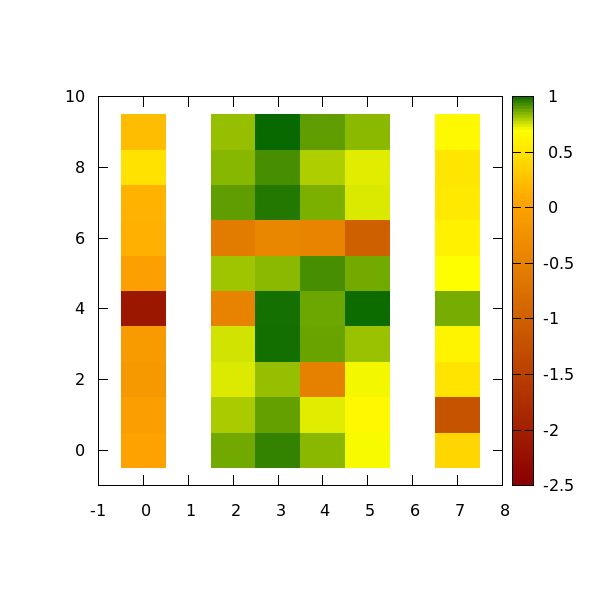
\includegraphics[width=0.75\textwidth]{common/img/matplot.png}
         \caption{Skalierte Ergebnisse der numerischen Lösung. Die Wert 1 steht für ein Ergebnis das zu 100\% dem wahren Wert entspricht und entsprechend zum Ende der Skala nimmt die Abweichung zu. Der Wert 0 steht bei dieser Skalierung für eine 100\%ige Abweichung. Kleinere Werte entsprechend für eine noch größere. }
         \label{fig:Matplot}
\end{figure}
%
\subsection{Software}
%
Da weiterhin keine neuen Messdaten vorliegen wurde an der Umsetzung des C++-Programms weitergearbeitet. Das in C++ geschriebene Programm läuft nativ auf dem Rechner des PRPS und wird ohnehin im späteren Verlauf des Projekts benötigt.
%
\subsubsection{Erstellung C++-Programm}
%
Das Programm gliedert sich in mehrere Unterbibliotheken, sodass diese Programmteile nach ihrer Fertigstellung in anderen Programmen eingesetzt werden können. Die Schnittstellen der einzelnen Programmteile stellen einfache CSV-Datein\footnote{CSV:=Comma Seperated Values} dar. Dabei werden die Ergebnisse der Berechnung in solche Datein geschrieben und von anderen Programmteilen erneut eingelesen. Das ermöglicht spätere Analyse der Daten und liefert eine einfache Möglichkeit der Protokollierung und Beurteilung eventuellen Fehlverhaltens der Software.
%
\subsubsection{Automatische Dokumentation}
%
In dieser Arbeit wird das automatische Dokumentationswerkzeug Doxygen \cite{Dox1} eingesetzt. Wie schon früher beschrieben\footnote{Pflichtenheft} ermöglicht das Werkzeug eine einfache und automatisierte Erstellung der Dokumentation aus Quellcodekommentaren.\\
Sobald eine aussagekräftige erste Version der Dokumentation erstellt werden kann, wird diese an den Wochenbericht angehängt.
%
\subsubsection{Stand des Programms}
%
Zum Ende der Woche ist es gelungen das Programm soweit zu entwickeln, dass alle möglichen Permutationen der Antennen und ihre zugehörigen Matrizen berechnet werden können. Die Matrizen wurden in eine separate Datei abgespeichert um sie anschließend mit den Ergebnissen der Excel Arbeitsmappe zu vergleichen. Das geschieht in der nächsten Woche.

%- Section 3 -----------------------------------------------------------------
\section{Probleme}
\label{Problems}
Keine neuen Probleme.
%
%- Appendix ------------------------------------------------------------------
%
%
%
\begin{appendix}

%----------------------------------------------------------------------------
%----------------------------------------------------------------------------
%----------------------------------------------------------------------------
\newpage

\begin{center}
	\huge{Anhänge}
\end{center}

\normalsize

%----------------------------------------------------------------------------
%----------------------------------------------------------------------------
%----------------------------------------------------------------------------
%\section{Modellumstellung}
%\label{trilateration_model_new}
%{
Abschließend soll das das bisher verwendete Modell umgeschrieben werden, damit die Allgemeingültigkeit darin enthalten ist.
\begin{align}
%
%\mathbf{0}&=\mathbf{A}\mathbf{x}-\mathbf{b}\\
%
\mathbf{A}&=
\left(
	\begin{array}{cccccc}
		x_k-x_0 & y_k-y_0 & z_k-z_0 & \sum_{i=1,j=0}^{k}(-a_1\delta_{ij}) &  -a_2\Theta_0 & \sum_{i=1,j=0}^{k}(a_2\Theta_k\delta_{ij})
	\end{array}
\right)\nonumber\\
%
\mathbf{x}&=
\left(
   \begin{array}{c}
	   x-x_0\\
	   y-y_0\\
	   z-z_0\\
	   n_0^2-n_k^2\\
	   n_0\\
	   n_k
   \end{array}
\right)\nonumber\\
%
\mathbf{b}&=
	\begin{array}{c}
		a_{0k}-a_{3kj} 
	\end{array}
	= c_{kj}'\nonumber
\end{align}
%
Dabei steht $\delta_{ij}$ für den bekannten Kronecker-Operator und bedeutet:
\begin{equation*}
\delta_{ij} = \begin{cases}1 ~\text{für}~ i=j\\ 0 ~\text{für}~ i\neq j\end{cases}
\end{equation*}
%
Im Expliziten sehen die Matrix $\mathbf{A}$ und der Vektor $\mathbf{b}$, für denn Fall $N'=3$ und $k=\{1,2,3\}$, wie folgt aus:
%
\begin{multline}
\mathbf{A}=\\
\left(
	\begin{array}{cccccccccc}
		x_1-x_0 & y_1-y_0 & z_1-z_0 & -a_1 & 0 & 0 & -a_2\Theta_0 & a_2\Theta_3 & 0 & 0 \\
		x_2-x_0 & y_2-y_0 & z_2-z_0 & 0 & -a_1 & 0 & -a_2\Theta_0& 0 & a_2\Theta_3 & 0 \\
		x_3-x_0 & y_3-y_0 & z_3-z_0 & 0 & 0 & -a_1 & -a_2\Theta_0& 0 & 0 & a_2\Theta_3
	\end{array}
\right) \nonumber
\end{multline}
%
\begin{equation}
\mathbf{x}=
\left(
	\begin{array}{c}
		x-x_0	\\
		y-y_0	\\
		z-z_0	\\
		n_0^2-n_1^2	\\
		(\dots)	\\
		n_0^2-n_3^2	\\
		n_0 \\
		n_1	\\
		(\dots)	\\
		n_3	
	\end{array}
\right)\nonumber
\end{equation}
%
\subsubsection{Bemerkungen - Finales Modell}
%
Das Ergebnis ist eine $3\times10$ Matrix und ein $1\times10$ Vaktor. Es ist möglich diesem Modell eine beliebige Anzahl an Antennen hinzuzufügen. Fügt man eine Antenne zur Berechnung hinzufügen würde sich die Matrix $\mathbf{A}$ um zwei Spalten und eine Zeile erweitern, der Vektor $\mathbf{x}$ analog um 2 Zeilen.

}

%----------------------------------------------------------------------------
%----------------------------------------------------------------------------
%----------------------------------------------------------------------------
\newpage
\begin{landscape}
	\section{Projektlaufplan KW 26}
	\label{sec:projectplan}
	\scalebox{.75}{
		\begin{ganttchart}[vgrid={draw=none,*1{gray, dashed}},
				hgrid=true,
				today=22,
				title height=1,
				y unit title=0.6cm,
				y unit chart=0.8cm,
				group right shift=0,
				group top shift=.3,
				group height=.3,
				milestone width=.8,
				group peaks={}{}{.2},
				incomplete/.style={fill=black!15}, %
				bar/.style={fill=white}, %
				today label={Heute},
				today rule/.style={dashed, thick}]{44}


\gantttitle{\textbf{2013}}{44} \\
\gantttitlelist{16,...,37}{2} \\
%-------------------------------------------------------------
\ganttgroup{Projekt Evaluation}{3}{14} \\
\ganttbar[progress=100, progress label font=\small\color{black!75},
	progress label anchor/.style={right=4pt}]{Installation der Umgebungen}{3}{6} \\
	
\ganttbar[progress=100, progress label font=\small\color{black!75},
	progress label anchor/.style={right=4pt},
	bar label font=\normalsize\color{black},
	name=rech]{Recherche}{3}{7} \\
	
\ganttmilestone[name=ms1]{Vorstellung der Ergebnisse}{7} \\
	
\ganttbar[progress=90, progress label font=\small\color{black!75},
	progress label anchor/.style={right=4pt},
	bar label font=\normalsize\color{black},
	name=pflichten]
	{Pflichtenheft}{5}{8} \\
	
\ganttmilestone[name=ms2]{Pflichtenheft fertig}{8} \\

\ganttbar[progress=90, progress label font=\small\color{black!75},
	progress label anchor/.style={right=4pt},
	bar label font=\normalsize\color{black},
	name=bNumVerf]
	{Einarbeitung num. Verfahren}{5}{16} \\

\ganttbar[progress=50, progress label font=\small\color{black!75},
	progress label anchor/.style={right=34pt},
	bar label font=\normalsize\color{black},
	name=bCMAES]
	{speziell CMA-ES}{7}{10} \\

\ganttmilestone[name=ms3]{Beurteilung num. Verfahren}{16} \\

\ganttlinkedbar[progress=10, progress label font=\small\color{black!75},
	progress label anchor/.style={right=34pt},
	bar label font=\normalsize\color{black}]
	{Shark Einarbeitung}{17}{18} \\

\ganttlinkedmilestone[name=ms7]{Abschluss Evaluation}{18} \\
	
%-------------------------------------------------------------
\ganttgroup{Erstellung Prototyp}{15}{26} \\
\ganttgroup{(optional)}{15}{18} \\
\ganttbar[progress=25, progress label font=\small\color{black!75},
	progress label anchor/.style={right=4pt},
	bar label font=\normalsize\color{black}]
	{(Entwurf digi. Filter)}{15}{15} \\

\ganttlinkedbar[progress=10, progress label font=\small\color{black!75},
	progress label anchor/.style={right=4pt},
	bar label font=\normalsize\color{black},
	name=bImpFPGA]
	{(Implementation FPGA)}{16}{18} \\

\ganttmilestone[name=ms4]{(Verifikation dig. Filter)}{18} \\
	
\ganttbar[progress=40, progress label font=\small\color{black!75},
	progress label anchor/.style={right=4pt},
	bar label font=\normalsize\color{black},
	name=bImplAlgo]
	{Implementation Algorithmus}{15}{26} \\

\ganttlinkedmilestone[name=ms5]{Implementation Done}{26} \\

%-------------------------------------------------------------
\ganttgroup{Verifikation}{27}{34} \\
\ganttbar[progress=10, progress label font=\small\color{black!75},
	progress label anchor/.style={right=4pt},
	bar label font=\normalsize\color{black},
	name=bVerf]
	{Durchf\"uhrung Verifikation}{27}{34} \\

\ganttlinkedmilestone[name=ms6]{Verifikation Done}{34} \\

%-------------------------------------------------------------
\ganttgroup{Projektdokumentation}{35}{42} \\

\ganttbar[progress=0, progress label font=\small\color{black!75},
	progress label anchor/.style={right=4pt},
	bar label font=\normalsize\color{black},
	name=thesis]
	{Thesis schreiben}{35}{42} \\
	
\ganttmilestone[name=msthesis,milestone label font=\color{red}, 
	milestone/.style={fill=red}]{Abgabe}{42}

%\ganttlink{ms7}{bImplAlgo}
\ganttlink{bImpFPGA}{ms4}
\ganttlink{bNumVerf}{ms3}
\ganttlink{bCMAES}{ms3}
\ganttlink{rech}{ms1}
\ganttlink{pflichten}{ms2}
\ganttlink{thesis}{msthesis}

	\end{ganttchart}
		}
\end{landscape}

%----------------------------------------------------------------------------

\end{appendix}


\newpage
%- Bibliography --------------------------------------------------------------
\bibliographystyle{ieeetr}
\bibliography{../bib/mathesis_collection1}

\end{document}